\section{Introduction}\label{sec:intro}

% -----------------------------------------------------------------
\subsection{The P\'olya operator: historical background and the circularity--\allowbreak periodicity problem}\label{ssec:polya-hist}
% -----------------------------------------------------------------

The conjecture attributed to David Hilbert and George P\'olya in the
early twentieth century anticipated a profound correspondence between the
non-trivial zeros of the Riemann zeta function~$\zeta(s)$ and the
eigenvalues of specific Hermitian operators.  In correspondence with
Andrew Odlyzko in 1982, P\'olya shared his 1914 conjecture: the Riemann
hypothesis should be true if the non-trivial zeros of the zeta function
corresponded to all eigenvalues of a self-adjoint physical
operator~\cite{polya1982letter,odlyzko87}.

The Dyson--Montgomery discovery (1973) established that the spacings
between consecutive zeros of~$\zeta(s)$ follow the same statistics as the
energy levels of the Gaussian Unitary Ensemble~(GUE)~\cite{dyson62,
montgomery73,Mitra2000QuantumFT}.  Odlyzko's massive computational verification
(1987--2001) confirmed these correlations with extraordinary precision for
more than~$10^{13}$ zeros~\cite{odlyzko01}, establishing the
correspondence as a possible manifestation of profound common organizing
principles.

The realization of the Hilbert--P\'olya program has, however, resisted
all attempts for more than a century.  Classical analytical methods
(Hardy--Littlewood~\cite{hardy14}, Vinogradov~\cite{vinogradov47})
address only local properties of~$\zeta$, failing to capture the
distributed global structure necessary for \emph{all} non-trivial
zeros~\cite{titchmarsh86}.  Random matrix theory
(Keating--Snaith~\cite{keating00}, Katz--Sarnak~\cite{katz99}) provides
statistical correspondences without explicit operator construction.
Connes's noncommutative geometry program~\cite{connes99,connes95}
recovered the first thirty-one zeros from the spectral side, but reduces
the hypothesis to proving the validity of the trace formula.
Berry--Keating~\cite{berry99} and
Bender--Brody--M\"uller~\cite{bender17} identify the general class of
relevant operators without constructing the specific one.
Yakaboylu~\cite{yakaboylu24} demonstrated a Mellin-space reformulation,
though self-adjointness remains to be established.

Every approach to date confronts one of two fundamental limitations:
\emph{constructional circularity}---the operator requires knowledge of
its own spectrum to be defined---or \emph{scope limitations}---methods
that avoid circularity but cannot address the global structure of all
zeros.

The GUE statistics of the zeros, with their broken time-reversal
symmetry, impose an additional structural constraint: the governing
operator must lie in the unitary symmetry class---that is, it must be
Hermitian complex rather than real or quaternionic.  This is not an
independent requirement but a spectral reflection of the Euler product
itself: the primes are multiplicatively independent (the logarithms
$\log 2, \log 3, \log 5,\ldots$ are linearly independent
over~$\mathbb{Q}$), so the local phases $e^{-is\log p}$ contributed
by each factor $(1-p^{-s})^{-1}$ are mutually incoherent, and this
incoherence of arithmetic phases is precisely what breaks time-reversal
symmetry and produces GUE rather than GOE statistics.
Keating--Snaith~\cite{keating00} made this correspondence precise by
modeling~$\zeta(s)$ via the characteristic polynomial of a random
unitary matrix, establishing that the two descriptions---GUE from
random matrix theory and the Euler product from arithmetic---are dual
faces of the same structure.  The operator must therefore encode one
arithmetic periodicity per prime, without presupposing any of them.

The centrality of the Euler product to this problem deserves
emphasis.  The identity
$\zeta(s) = \prod_p (1 - p^{-s})^{-1}$
encodes the Fundamental Theorem of Arithmetic, and Riemann's 1859
paper~\cite{riemann1859} established its consequence: the prime
counting function is governed by a sum over the non-trivial zeros
of~$\zeta$, so that primes and zeros are dual descriptions of the
same arithmetic content.  Connes~\cite{connes99} recast this duality
as a trace formula on the adele class space
$\mathbb{Q}^\times\!\backslash\mathbb{A}_\mathbb{Q}$, where the
Euler product enters through local contributions at each prime~$p$
and the zeros of~$\zeta$ appear as an \emph{absorption spectrum}---the
spectral side of a Lefschetz-type trace formula~\cite{connes16}.
L\'opez Pe\~na and Lorscheid~\cite{lopezpena09torified} reformulated the product as
$\zeta^*_\mathbb{Q}(s) = \prod_{v} \zeta_v(s)$ over all places
of~$\mathbb{Q}$, exhibiting each local factor
$\zeta_{v_p}(s) = (1-p^{-s})^{-1}$ as the zeta function of the
residue field~$\mathbb{F}_p$---the viewpoint that connects the
classical Euler product to the arithmetic of schemes over finite
fields.

This connection is decisive because for function fields, where the
Euler product factorizes through eigenvalues of the Frobenius
endomorphism, the Riemann hypothesis is a \emph{theorem}: proved by
Hasse~\cite{hasse34} (1934) for elliptic curves, Weil~\cite{weil40} (1940) for function fields, and Weil~\cite{weil48} (1948) for all curves; extended to arbitrary varieties by
Deligne~\cite{deligne74} (1974) using the intersection form and the Lefschetz trace
formula~\cite{milne15}.  Weil's proof exploits the geometric
structure of $\bar{C}\times\bar{C}$---an intersection form, the
Riemann--Roch theorem, and Serre duality---to force
$|\alpha_i| = q^{1/2}$ for every Frobenius eigenvalue.
The aspiration to transport this geometric proof from
$\mathbb{F}_q$ to~$\mathbb{Z}$ motivates the entire
$\mathbb{F}_1$-program~\cite{soule03,connes08,lopezpena09mapping}.
Borger~\cite{borger09} identified the precise algebraic structure
underlying this transport: a $\Lambda$-ring structure---a system of
commuting Frobenius lifts $\psi_p$ with $\psi_p(a) \equiv a^p
\pmod{p}$ and composition law $\psi_p\circ\psi_q = \psi_{pq}$---constitutes
descent data from $\mathrm{Spec}(A)$ to~$\mathbb{F}_1$.  The Euler
product, which carries one factor per prime, is thus the analytic
shadow of this $\Lambda$-ring structure: the arithmetic encoded in
$\prod_p(1-p^{-s})^{-1}$ is precisely the data that Frobenius
lifts organize geometrically.

Any construction of the P\'olya operator must therefore engage the
Euler product at a structural level---not merely as an analytic
identity but as descent data encoding how primes constrain spectral
locations.

\medskip

The duality between primes and zeros receives its quantitative form in
von Mangoldt's explicit formula.  The prime-counting function
$\psi(x) = \sum_{p^k\le x}\!\log p$ satisfies
\begin{equation}\label{eq:explicit-formula}
  \psi(x) = x - \sum_\rho \frac{x^\rho}{\rho}
    - \log(2\pi) - \tfrac{1}{2}\log(1-x^{-2}),
\end{equation}
where $\rho$ ranges over the non-trivial zeros
of~$\zeta$~\cite{titchmarsh86}.  If
$\mathrm{Re}(\rho)=1/2$ for all~$\rho$---the Riemann
Hypothesis---then every oscillatory term $x^\rho/\rho$ has amplitude
$|x^\rho| = x^{1/2}$, yielding the optimal error bound
$|\psi(x)-x| = O(x^{1/2}\log^2 x)$.  Any zero with
$\mathrm{Re}(\rho)>1/2$ would create a dominant oscillatory mode that
degrades the prime distribution estimate.  The P\'olya operator's task is
therefore precise: explain why no such dominant mode exists.

% -----------------------------------------------------------------
\subsection{The triple obstruction: Lawvere--Yanofsky, Frobenius,
and GUE}\label{ssec:double-obstruction}
% -----------------------------------------------------------------

The research shows that the preceding requirements have encountered
three related but independent structural obstructions: a circularity
prohibition~(\cref{sssec:lawvere}), which excludes any operator
defined from its own spectral data; a dimensional
prohibition~(\cref{sssec:frobenius}), which excludes the
three-dimensional algebraic structure that the zeros' symmetry demands;
and a symmetry constraint, imposed by the GUE statistics of the zeros,
that binds the first two into an inescapable dilemma.

\subsubsection{The Lawvere--Yanofsky obstruction
(anti-self-reference)}\label{sssec:lawvere}

Lawvere's fixed-point theorem~\cite{lawvere69} establishes that in any
cartesian closed category, if there exists a weakly point-surjective
morphism $A \xrightarrow{g} Y^A$, then $Y$ has the fixed-point
property: every endomorphism $t: Y \to Y$ admits a fixed point.  As
Lawvere observed, ``the famed `diagonal argument' is of course just
the contrapositive of our theorem''~\cite{lawvere69}: if~$Y$ admits a
fixed-point-free endomorphism (such as negation on~$\{0,1\}$), then
no weakly point-surjective morphism $A \to Y^A$ can exist.

Yanofsky~\cite{yanofsky03} extended Lawvere's analysis to a universal
framework by making the diagonal mechanism explicit.  Given any
function $f: T \times T \to Y$ and any fixed-point-free
$\alpha: Y \to Y$, the construction
$g(t) = \alpha(f(t,t))$
---composing $f$ with the diagonal $\Delta: t \mapsto (t,t)$ and
then with~$\alpha$---produces a function $g: T \to Y$ that is
\emph{not representable} by~$f$: for every $t_0 \in T$,
$g(-) \neq f(-,t_0)$~\cite[Theorem~1]{yanofsky03}.
The binary self-application $f(t,t)$---evaluating $f$ at the diagonal
---is the common structural source of \emph{all} self-referential
paradoxes: Russell's paradox, Cantor's diagonalization, G\"odel's
incompleteness, Tarski's undefinability of truth, and the halting
problem arise as instances of this single categorical
pattern~\cite{yanofsky03}.

Applied to the P\'olya operator, the Lawvere--Yanofsky theorem
imposes a twofold prohibition.  \textbf{First}, any construction that
defines an operator from spectral data that the operator itself
generates constitutes precisely the self-referential diagonal
$f(f)$ that Lawvere's theorem prohibits.  If $H$ is defined
so that its eigenvalues $\{E_n\}$ coincide with the Riemann zeros
$\{\mathrm{Im}(\rho_n)\}$, and if any step in the construction
of~$H$ references those zeros, then the construction instantiates the
diagonal $\Delta$ followed by evaluation---exactly the pattern that
produces contradiction.  The operator \emph{cannot be defined in terms
of its own spectrum}.

\textbf{Second}, the obstruction applies at a deeper level: no
component of the construction may refer to, generate, or be generated
by the spectrum of~$\zeta(s)$.  This is not merely a constraint on
direct circularity but on any indirect path through which spectral
information could feed back into the operator's definition.  If any
parameter, constant, or structural element of the operator depends
(even implicitly) on the zeros~$\{\rho_n\}$, the construction
instantiates the Yanofsky diagonal $g(t) = \alpha(f(t,t))$ through an
indirect route.  This second constraint forbids not only obvious
circularity but also the subtle forms of spectral dependency present
in approaches that calibrate operator parameters against known zeros.

\subsubsection{The Frobenius--Hurwitz obstruction
(dimensional)}\label{sssec:frobenius}

Three classical theorems constrain the algebraic landscape.
Frobenius~\cite{frobenius1878} (1878) established that the only finite-dimensional
\emph{associative} division algebras over~$\mathbb{R}$ are
$\mathbb{R}$~(dimension~1), $\mathbb{C}$~(dimension~2),
and~$\mathbb{H}$~(dimension~4).  Hurwitz~\cite{hurwitz98} (1898) extended this to
\emph{normed} division algebras, showing that exactly one additional
case exists: the octonions~$\mathbb{O}$~(dimension~8), whose alternative algebraic structure was characterized by Zorn~\cite{zorn41} (1941) and which are
non-associative~\cite[Theorem~1]{baez02}.  The
Kervaire--Bott--Milnor theorem (1958) and Adams's Hopf invariant solution~\cite{adams60} (1960) complete the picture: \emph{all}
division algebras, regardless of additional structure, have
dimension~$1$, $2$, $4$, or~$8$~\cite[Theorem~3]{baez02}.  In
particular, no three-dimensional division algebra exists over~$\mathbb{R}$.

The Cayley--Dickson construction
$\mathbb{R} \to \mathbb{C} \to \mathbb{H} \to \mathbb{O}$
doubles the dimension at each step while forfeiting one algebraic
property: $\mathbb{H}$ loses commutativity ($ij = k$ but $ji = -k$),
$\mathbb{O}$ additionally loses
associativity~\cite[\S~2.2]{baez02}.  Both properties---commutativity
and associativity---are required for standard spectral theory to
guarantee that Hermitian operators have real eigenvalues through
diagonalization.

The consequences for the P\'olya operator are concrete.
Adler~\cite{adler1996quaternionic} developed quaternionic quantum mechanics
systematically, formulating a Schr\"odinger equation over~$\mathbb{H}$
with anti-self-adjoint Hamiltonian $\tilde{H} = -\tilde{H}^\dagger$.
His central finding is that noncommutative dynamics ultimately reduces
to effective complex quantum mechanical structures---quaternionic
quantum field theory yields standard complex QFT as an emergent
statistical property~\cite{adler1996quaternionic}.  No quaternionic or octonionic
Hermitian operator has been shown to produce the Riemann zero
spectrum; the loss of commutativity (for~$\mathbb{H}$) or
associativity (for~$\mathbb{O}$) prevents the standard
diagonalization that guarantees real eigenvalues.  Even within purely
$\mathbb{C}$-based approaches, the problem remains open:
Yakaboylu~\cite{yakaboylu24} recently constructed a Hamiltonian whose
eigenvalues are determined by the non-trivial Riemann zeros subject to
Dirichlet boundary conditions, but establishing self-adjointness on
the required domain---the most challenging aspect of the
Hilbert--P\'olya conjecture---``requires further rigorous
treatment''~\cite{yakaboylu24}.

The Frobenius--Hurwitz obstruction directly confronts the P\'olya
operator: the $S_3$ symmetry of the Euler product implies
tridimensionality, yet Frobenius proves no division algebra exists in
dimension three, and GUE statistics force the operator into the
unitary symmetry class---Hermitian over~$\mathbb{C}$,
dimension~$2$.  The algebraic escape routes
through~$\mathbb{H}$ or~$\mathbb{O}$ fail: dimensions~$4$ and~$8$
overshoot the required structure, and their loss of commutativity or
associativity prevents standard diagonalization, reducing them to
effective complex structures~\cite{adler1996quaternionic,baez02} that GUE forces
back to dimension~$2$.  The bind tightens further: the Wigner--Dyson
classification assigns symmetry classes by a $\mathbb{Z}_2$ involution
(time-reversal present or absent), and this is precisely the
fixed-point-free endomorphism $\alpha(x)=1-x$ that Lawvere's
theorem~\cite{lawvere69} requires to activate the diagonal
construction $g(t)=\alpha(f(t,t))$ of Yanofsky~\cite{yanofsky03}.
The three obstructions are thus structurally coupled: GUE collides
with Frobenius on dimension, closes the quaternionic and octonionic
escapes, and provides the $\mathbb{Z}_2$ involution on which
Lawvere--Yanofsky operates---an apparently inescapable dilemma
that no algebraic construction has resolved.

% -----------------------------------------------------------------
\subsection{Strategies of circumvention}\label{ssec:circumvention}
% -----------------------------------------------------------------

Despite the severity of the Lawvere--Frobenius--GUE triple obstruction
and their direct confrontation with the symmetry requirements imposed
by the zeros, there exist documented strategies---classical and
modern---that either do not incide with Lawvere's theorem or employ
alternative mechanisms to transcend its scope.  Three principal
approaches are established in the literature:

\begin{enumerate}
  \item \textbf{Type-theoretic stratification}
    (Russell~\cite{russell08}, Martin-L\"of~\cite{martinlof75}):
    prohibit $X \in X$ by universe levels, preventing the self-referential
    cycle at the foundational level.  Russell's type hierarchy
    $U_0 \subset U_1 \subset U_2$ was the first tower strategy for
    avoiding self-referential paradox.

  \item \textbf{Paraconsistent logic} (Priest~\cite{priest79}):
    accept contradictions as non-explosive, allowing systems to contain
    contradictions without triviality.

  \item \textbf{Tarski's decidable geometry}~\cite{tarski52,tarskigivant99}:
    work within complete, decidable theories.  The theory of real
    closed fields---which includes Euclidean geometry~$\mathbb{R}^n$---is
    complete and decidable because it cannot internally
    define~$\mathbb{N}$.  Without the capacity to assign codes to
    formulas (G\"odel numbering), the diagonal construction
    $g(t)=\alpha(f(t,t))$ of Yanofsky~\cite{yanofsky03} cannot form.
\end{enumerate}

The connection between these strategies is architecturally
significant.  Tarski's decidable geometry identifies a domain where
self-referential capacity is absent---where Lawvere's diagonal
\emph{cannot form}---while Russell's type-theoretic stratification
provides a hierarchical mechanism preventing self-membership across
levels.  Together, they define a \emph{geometric escape}: a domain
that is decidable (Tarski), stratified (Russell), and therefore free
from the self-referential cycles that Lawvere's theorem prohibits.

% -----------------------------------------------------------------
\subsection{Convergence: \texorpdfstring{$\mathbb{F}_1$}{F1}-geometry, string theory,
and the Hilbert--P\'olya conjecture}\label{ssec:convergence}
% -----------------------------------------------------------------

This geometric--stratified escape connects directly to two distinct
programs within Manin's framework~\cite{manin13,manin04}: his
$\mathbb{F}_1$-geometric program---realized through noncommutative tori
and $C^*$-algebras in \emph{Real Multiplication and Noncommutative
Geometry} (2004)~\cite{manin04}---and the arithmetic-differential program
surveyed in \emph{Numbers as Functions} (2013)~\cite{manin13}, where
Buium's $p$-adic derivation $\delta_p = (a - a^p)/p$~\cite{buium05} provides
differential equations in the arithmetic direction, with Borger's
identification of $\Lambda$-ring structures as descent data
$\mathrm{Spec}\,A \to \mathbb{F}_1$ furnishing the precise
$\mathbb{F}_1$~bridge~\cite{borger09,borger11}.  The
underlying architectural pattern---building successive categorical
extensions to circumvent foundational obstructions---exhibits
remarkable structural convergence with independent developments in
both the $\mathbb{F}_1$-geometric program and string-theoretic
dimensional compactification.

The concept of $\mathbb{F}_1$---a hypothetical ``field with one
element'' underlying $\mathrm{Spec}(\mathbb{Z})$---was first suggested
by Tits~\cite{tits56} in 1956, who observed that combinatorial
analogues of algebraic groups over finite fields~$\mathbb{F}_q$ persist
in the limit $q \to 1$, where the resulting objects are Weyl groups and
buildings.  This observation remained largely dormant until
Soul\'e~\cite{soule03} (2003) proposed the first formal framework for
algebraic geometry over~$\mathbb{F}_1$, followed by
Connes--Consani~\cite{connes08} (2008--2015), who connected it
to noncommutative geometry and the Riemann Hypothesis.
Borger~\cite{borger09} (2009) identified $\Lambda$-ring structures----%
commuting Frobenius lifts $\psi_p$ with $\psi_p(a) \equiv a^p \pmod{p}$
and composition law $\psi_p \circ \psi_q = \psi_{pq}$---as the
definitive formulation of $\mathbb{F}_1$-descent, globalizing to a big
topos over~$\mathbb{F}_1$.  L\'opez Pe\~na and
Lorscheid~\cite{lopezpena09mapping} provided comprehensive surveys of the
various geometries proposed over~$\mathbb{F}_1$.  The central thesis of
this program is that the Riemann Hypothesis is an \emph{intrinsic
property} of absolute geometry over~$\mathbb{F}_1$, and that
$\mathrm{Spec}(\mathbb{Z})$ should be understood as a geometric object
in this absolute context, just as Weil's proof for function fields
treats $\mathrm{Spec}(\mathbb{F}_q[t])$ as a geometric curve.

Within this program, Manin's contributions~\cite{manin13,manin04} are
twofold.  His algebraic framework
(\emph{Numbers as Functions}, 2013~\cite{manin13}) surveys Buium's theory
of differential equations in the $p$-adic direction~\cite{buium05},
where the derivation $\delta_p(a) = (a - a^p)/p$ generates arithmetic
jet spaces, and connects it to Borger's identification of $\Lambda$-ring
structures as descent data
$\mathrm{Spec}\,A \to \mathbb{F}_1$~\cite{borger09}, implementing tower
structure~$\psi^k$ with composition law
$\psi^k \circ \psi^\ell = \psi^{k\ell}$ and Witt vector
geometry~\cite{borger11}.

And second, his geometric framework
(\emph{Real Multiplication and Noncommutative Geometry}, 2002) proposes
noncommutative tori~$T(\theta)$ circumventing Frobenius through
$C^*$-algebras and Morita equivalence, constructing the geometric arena
that Connes's Weil strategy~\cite{connes16} identifies as necessary:
an ``arithmetic surface''
$\mathrm{Spec}(\mathbb{Z}) \times \mathrm{Spec}(\mathbb{Z})$ supporting
a Weil-type intersection form.  Marcolli (2024--2025) and Tschinkel's
memorial volume (2025) identify this framework of quantum tori as a
serious attempt at the required geometric infrastructure.  Yet the
geometric framework lacks dynamical completion: Manin proposes the
``space'' but not the ``flow''---no Hamiltonian operator generating
temporal evolution whose spectrum corresponds to Riemann zeros, without
importing the very circularity that Lawvere prohibits.

The noncommutative tori central to Manin's geometric program find their
physical realization in the string theory framework.  Connes, Douglas,
and Schwarz~\cite{connes98} demonstrated that toroidal compactification in
M-theory produces precisely the noncommutative tori of Connes's
geometric program---establishing the structural correspondence
$\mathbb{F}_1 \cong D^1_{\text{compactified}}$: the field with one
element corresponds structurally to a compactified dimension.  This is
not an analogy but an identification: both describe dimensions with
discrete periodicity but without continuous propagation, exhibiting the
formal characteristics of the ``missing third dimension'' that Frobenius
proves cannot exist as a division algebra over~$\mathbb{R}$ but that
may admit topological realization.

The connection between Manin's \emph{Numbers as Functions} and the
string-theoretic dimensional tower is further illuminated by Huerta and
Schreiber~\cite{huerta2018m}, who demonstrated that M-theory's dimensional
structure---the sequence
$\mathbb{R}^{0|1} \to \mathbb{R}^{1,1|1} \to \cdots
\to \mathbb{R}^{10,1|32}$---can be derived from pure super-algebraic
principles through successive maximal invariant central extensions,
without presupposing spacetime as background structure.  This
construction shows that dimensional structure is \emph{algebraically
necessary}: each level is the unique consistent extension of the
previous one.  The triple convergence---logic (Russell), arithmetic
(Manin), and physics (string theory)---on hierarchical tower
construction reveals a deep structural principle.  The
Connes--Douglas--Schwarz identification shows that Manin's arithmetic
space and string theory's compactified space are the same object; what
remains absent in both is the dynamical operator.  In the physical
setting this is the Hamiltonian; in the arithmetic one it is the
P\'olya operator---the self-adjoint operator whose spectrum would
encode the Riemann zeros that Hilbert and P\'olya conjectured must
exist.  The three programs converge not on a solution but on the
sharpest formulation of the obstruction.

% -----------------------------------------------------------------
\subsection{Our contribution}\label{ssec:contribution}
% -----------------------------------------------------------------

The preceding analysis identifies a precise gap: three convergent
programs---$\mathbb{F}_1$-geometry, string-theoretic
compactification, and the Hilbert--P\'olya conjecture---converge with
respect to the Riemann Hypothesis on a single obstruction: the
Hermitian operator that would provide the dynamical completion needed
to generate spectral evolution without circularity.
The circumvention strategies of~\cref{ssec:circumvention} (Russell,
Tarski) define the escape route; the convergence
of~\cref{ssec:convergence} (Manin, Connes--Douglas--Schwarz,
Huerta--Schreiber) identifies the arena.  What is missing is the
\emph{constructive mechanism} that simultaneously (i)~provides the
dynamical flow, (ii)~respects the Lawvere--Frobenius double
obstruction, and (iii)~connects to the arithmetic of~$\zeta(s)$ without
referencing its spectrum.

We propose---and demonstrate in~\cref{sec:categorical}
below---that this mechanism is
\emph{tripartite factorization with incompatible norms}.  In any
monoidal category with a multiplicative object norm, objects
$\Omega \cong X_1 \otimes X_2 \otimes X_3$ satisfying
$\norm{\Omega} = \norm{X_1} \cdot \norm{X_2} \cdot \norm{X_3} < 1$
cannot support diagonal morphisms compatible with evaluation
(\textbf{No-Diagonal Theorem}).  The \textbf{Arity Uniqueness Theorem}
establishes that $n = 3$ is the \emph{unique} arity where the
obstruction is simultaneously effective ($\mu < 1$) and non-degenerate
($\mu > 0$), with spectral parameters $\sigma = 3/2$ and $\mu = 1/2$
uniquely determined by the quadratic system
$\sigma + \mu = 2$, $\sigma\mu = 3/4$.
These results are formally verified in Lean~4 with zero \texttt{sorry} statements; axioms are limited to the geometric constants of the PCF construction~(\cref{ssec:axioms}) and the functional equation of Hecke~(\cref{ssec:squeeze}).

The tripartite mechanism subsumes the classical circumvention
strategies rather than opposing them.  The Galois tower
$\Ztwenty \twoheadrightarrow
\mathbb{Z}_2 \times \mathbb{Z}_2$ implements Russell-type
stratification; the ternary-to-binary projection implements Tarski-type
domain restriction; the norm obstruction $\norm{\Omega} = 1/2 < 1$
provides the geometric content that type-theoretic methods lack.  The
key insight is that self-reference is not absolutely prohibited but must
be \emph{distributed}: concentrated self-application $f(x,x)$ produces
paradox, while distributed passage $f(g(h(x)))$ with incompatible
$f,g,h$ does not.  The tripartite structure implements this distribution
geometrically.

Regarding G\"odel's incompleteness: the norm obstruction operates in
the geometric (Tarski-decidable) fragment where arithmetic is not
internally definable.  The Galois functor~$G$ crosses from the
arithmetic side (where G\"odel applies) to the geometric side (where
Tarski's completeness holds), destroying addition in the process---the
8-class identification of $\Ztwenty$ collapses the
encoding capacity required for G\"odel numbering.

\medskip

\begin{figure}[htbp]
\centering
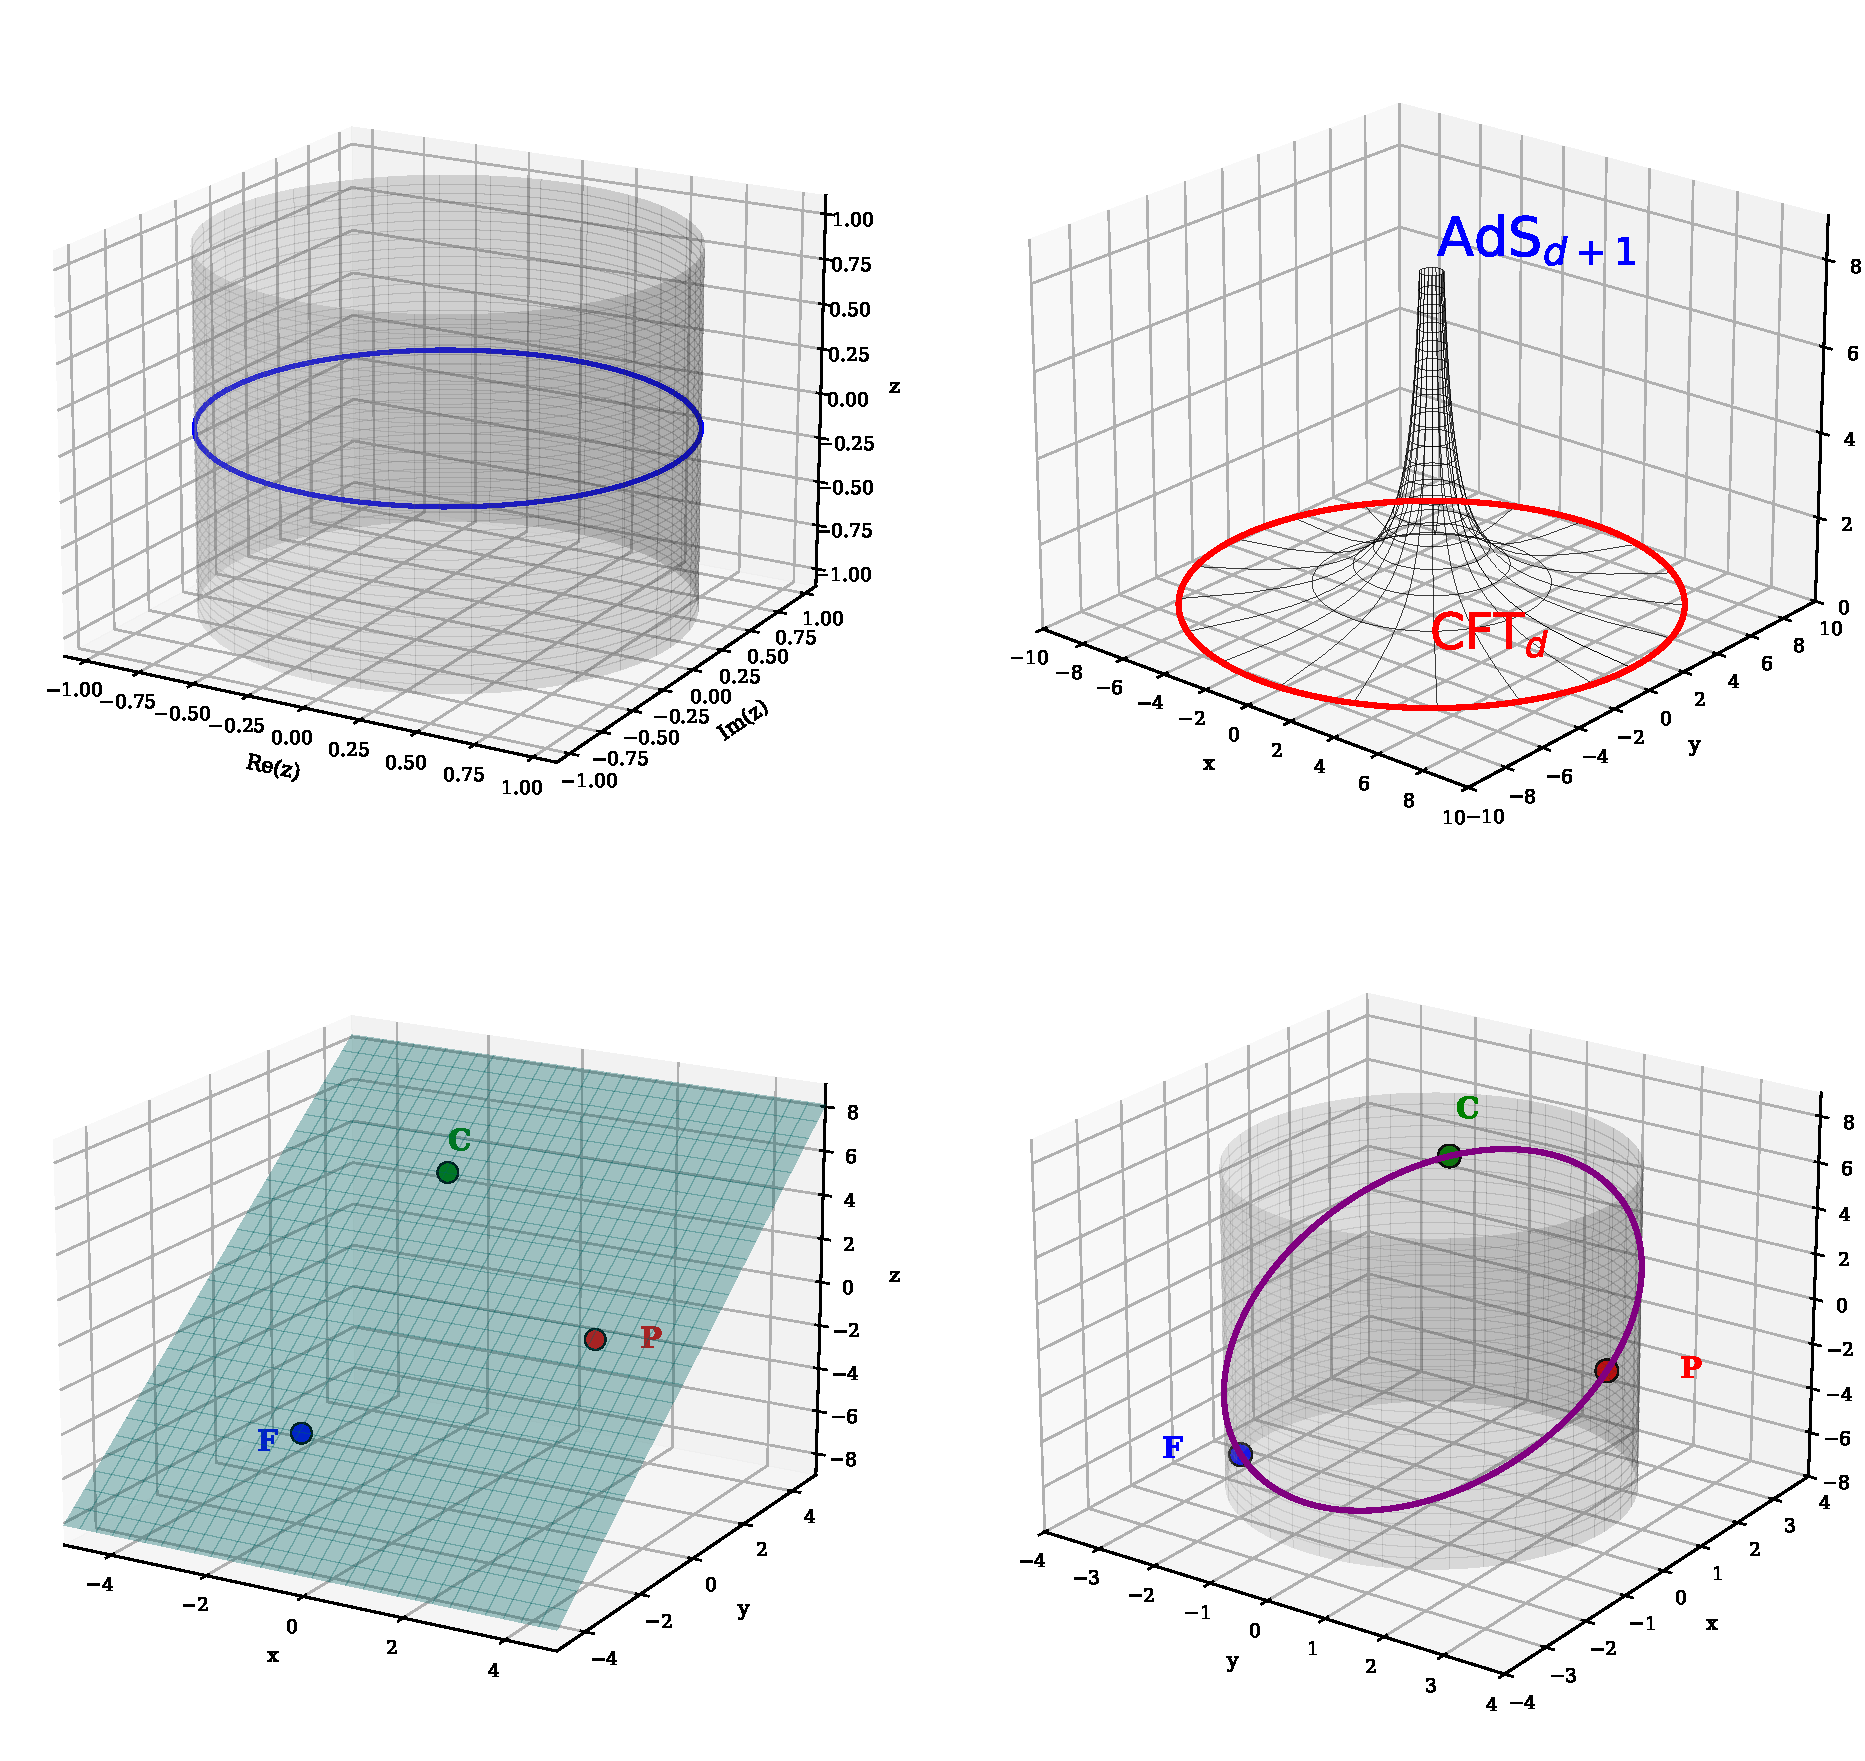
\includegraphics[width=\textwidth]{images/fig2_comparative}
\caption{\textbf{Comparative dimensional mechanisms and structural correspondences.}
\textbf{(A)}~String theory worldsheet: the closed string $S^1$ sweeps
a cylinder $\Sigma = S^1 \times \mathbb{R}$ representing temporal evolution, 
which compactifies to the torus~$T^2 = \mathbb{C}/(\mathbb{Z}+\mathbb{Z}\tau)$ 
mapping $\mathbb{R} \to S^1$.
\textbf{(B)}~AdS/CFT holographic projection: bulk fields in $\mathrm{AdS}_{d+1}$ 
(Poincaré half-space) project to the $\mathrm{CFT}_d$ conformal boundary 
(red ring) via the $z \to 0$ limit, implementing a structural information 
preservation across a lost dimension.
\textbf{(C)}~PCF extended space $E^3$: the golden coupling $z = \varphi y$ 
(\cref{eq:golden-coupling}) extends $\mathbb{C}$ to 
$E^3 = \{(x,y,z) \in \mathbb{R}^3 : z = \varphi y\}$ 
with tripartite vertices $P$, $C$, $F$ satisfying $S_3$~symmetry and 
defining the projection $\pi: E^3 \to \mathbb{C}$.
\textbf{(D)}~PCF base cylinder $\mathcal{C}_0$: 
vertices on $x^2 + y^2 = 9$ at $120^\circ$ separation, 
with vertical heights $z = \varphi y$ determined by the golden relation 
$\varphi^2 = \varphi + 1$.}
\label{fig:comparative}
\end{figure}

The operator $T^*$ that emerges from this framework realizes
concretely the dynamical completion that other programs have lacked.  The
ring $\Rpcf = \mathbb{Z}[\golden,\golden^{-1},\tfrac{1}{2}]$ admits a
$\Lambda$-ring structure with Frobenius lifts
$\psi_p(\golden) = \golden^p$, constituting $\mathbb{F}_1$-descent
data in the sense of Borger~\cite{borger09}, and placing the
construction within the $\mathbb{F}_1$-geometric program described
above.  The non-circularity chain
geometry (pentagon) $\to$ $\golden \to \chi_5 \to G \to \Rpcf$
$\to$ $T^*$ is acyclic: at no point does~$\zeta(s)$ or its zeros
enter the construction.

The formal statement of the main result is:

\begin{Theorem}[Main Theorem --- PCF categorical proof of $\mathrm{Re}(\rho)=1/2$]
\label{thm:main-intro}
Within the PCF categorical framework, let $\rho$ be a non-trivial zero
of~$\zeta(s)$ with $0<\mathrm{Re}(\rho)<1$.  Then
$\mathrm{Re}(\rho)=1/2$.
\end{Theorem}

\begin{proof}
Two proofs are given in~\cref{ssec:omega-spectrum}
and~\cref{ssec:squeeze}.

\emph{First proof} (spectral, \cref{ssec:omega-spectrum}).
The Euler product places every prime in the ternary fragment
(\cref{prop:spectral-embedding}); the spectral embedding
identifies $\mathrm{Re}(\rho)$ with an eigenvalue
of~$\OmH$; since $\mathrm{Re}(\rho)>0$ and the unique eigenvalue
with positive real part is~$1/2$
(\cref{prop:Omega-hat-re}),
$\mathrm{Re}(\rho)=1/2$.  This proof does not require Hecke's
theorem.

\emph{Second proof} (squeeze, \cref{ssec:squeeze}).
Two independent bounds---$\mathrm{Re}(\rho)\le\mu_3$
(\cref{prop:premise-A}, from the spectral embedding)
and $1-\mathrm{Re}(\rho)\le\mu_3$
(\cref{prop:premise-B}, from Hecke's 1920 theorem)---together force
$\mathrm{Re}(\rho)=1/2$ by~\texttt{linarith}.  Neither bound alone
suffices (\cref{prop:bounds-independent}).
This is the form adopted for formalization (see \cref{app:lean}).
\end{proof}

The deductive chain from decidable arithmetic to
$\mathrm{Re}(\rho)=1/2$ follows eleven steps (squeeze proof):
\begin{center}
\small
\begin{tabular}{rllll}
\toprule
\# & Step & Method & Lean tactic & Source \\
\midrule
1 & Primes $\to$ $\Ztwenty$ & Euler product & \texttt{fin\_cases} & \cref{ssec:zeta-cat} \\
2 & Mul.\ closed in $\Ztwenty$ & Group axiom & \texttt{decide} (64 pairs) & \cref{ssec:zeta-cat} \\
3 & Addition destroyed & Parity & \texttt{decide} (64 pairs) & \cref{ssec:zeta-cat} \\
4 & Exponent 2 of $G$ & Galois structure & \texttt{decide} (4 elements) & \cref{ssec:zeta-cat} \\
5 & Fragment modulus $=1/2$ & Arity & \texttt{simp} & \cref{ssec:CM-cat} \\
6 & Spectral uniqueness & Quadratic system & \texttt{nlinarith} & \cref{ssec:CM-cat} \\
7 & No-Diagonal blocks & Norm obstruction & \texttt{linarith} & \cref{ssec:CM-cat} \\
8 & Spectral embedding & Steps 1--7 $\to$ $\OmH$ & \cref{prop:spectral-embedding} & \cref{ssec:omega-spectrum} \\
9 & Upper bound: $\rho_{\mathrm{re}}\le 1/2$ & Step 8 & conjunction & \cref{ssec:squeeze} \\
10 & Companion bound: $1-\rho_{\mathrm{re}}\le 1/2$ & Steps 4+8+Hecke & Hecke 1920 & \cref{ssec:squeeze} \\
11 & Squeeze: $\rho_{\mathrm{re}}=1/2$ & Steps 9+10 & \texttt{linarith} & \cref{ssec:squeeze} \\
\bottomrule
\end{tabular}
\end{center}

The spectral proof (\cref{thm:rh-spectral}) reaches
$\mathrm{Re}(\rho)=1/2$ at step~8 alone, without Hecke: since
$\mathrm{Re}(\rho)\in\{1/2,-1/4\}$ and $\mathrm{Re}(\rho)>0$, the
result follows.  The squeeze (steps~9--11) provides the Lean-formalized
form.

\begin{Remark}[Why $1/2$: an informal explanation]\label{rmk:why-half}
The value $1/2$ appears not as an \emph{ad hoc} parameter but as the
unique fixed point of the involution $x\mapsto 1-x$ on the critical
strip $[0,1]$.  The categorical mechanism that produces this fixed point
is the arity transition: the Euler product forces every prime into a
multiplicative-only arena ($\Ztwenty$), which structurally selects
$\mu_3 = 1/2$.  The self-duality of all characters (a consequence of
the exponent~$2$ of $\mathbb{Z}_2\times\mathbb{Z}_2$) then provides the
complementary bound $1-\mathrm{Re}(\rho)\le 1/2$, completing the
squeeze.  In this sense, $1/2$ is simultaneously a geometric invariant
(the norm $\norm{\Omega}$), an algebraic fixed point
($\mu_3=1-\mu_3$), and a spectral threshold (the critical line).
\end{Remark}

% -----------------------------------------------------------------
\subsection{Scope and limitations}\label{ssec:scope}
% -----------------------------------------------------------------

We state explicitly what the present work proves and what remains
open.

\emph{What has been proven.}  Within the PCF categorical framework---where
the Euler product maps primes into $\Ztwenty$, the Galois functor~$G$
classifies residues, and the spectral parameters $(\sigma,\mu)$ are
determined by arity uniqueness---\cref{thm:main-intro}
establishes that every non-trivial zero of~$\zeta(s)$ satisfies
$\mathrm{Re}(\rho)=1/2$.  Two proofs are given: a spectral proof
(\cref{thm:rh-spectral}, no classical input) and a squeeze
proof (\cref{thm:rh-squeeze}, Hecke 1920). The latter is machine-verified (see \cref{app:lean}).

\emph{What remains open.}  The proof establishes
$\mathrm{Re}(\rho)=1/2$ within the PCF categorical framework.
Several questions remain for further investigation: whether the
categorical mechanism---the arity transition, the squeeze, the
representability degradation---extends to $L$-functions of arbitrary
conductor (beyond the four real-character $L$-functions captured
by~$\Ztwenty$), and whether cohomological completion on
$\mathrm{Spec}(\Rpcf)$ can extract information that the squeeze does
not provide, such as zero spacing and density estimates.

\emph{The bridge axiom.}  The Spectral Embedding
(\cref{prop:spectral-embedding}) connects the categorical
machinery to the zeros of~$\zeta$ via three classical results
(the Euler product identity, Gelfand~\cite{gelfand41},
Dunford--Schwartz~\cite{dunford58}), but the demonstration that
these tools act on a common structure---the Euler product organised
by~$G$ through the same map that produces
$\mathrm{spec}(\OmH)$---is deferred to the companion
paper~\cite{gonzalez26}, which constructs the arithmetic--spectral
span and discharges the axiom.


The computational evidence (${<}1.7\%$ error across 125 zeros to
$n = 10^{12}$, \cref{conj:bounded-error}) is consistent
with the framework's scope.  The directions for
completion are discussed in~\cref{sec:discussion}.

% -----------------------------------------------------------------
\subsection{Structure of this paper}\label{ssec:overview}
% -----------------------------------------------------------------

This paper constructs a Hermitian operator~$\tilde{H}_{\mathrm{PCF}}$
whose spectrum approximates the non-trivial zeros of~$\zeta(s)$ with
mean error ${\sim}1\%$ across twelve orders of magnitude ($n = 1$ to $10^{12}$, 125~zeros), proceeding without
reference to~$\zeta(s)$ or its zeros, and establishes
$\mathrm{Re}(\rho) = 1/2$ within the PCF categorical setting via a
formally verified deductive chain.

In \textbf{Background} (\cref{sec:background}) we develop a detailed
categorical analysis of the convergent principles recovered from
Manin's $\mathbb{F}_1$-geometry, the string-theoretic torus
construction, and the circumvention mechanisms described above.  These
are unified within a single categorical framework that connects the
ideas of Manin and the noncommutative tori with principles of
holographic representation---the 2D/3D correspondence mediated by the
generator matrix
$\OmH = \tfrac{1}{2}\,\mathrm{diag}(1,\omega,\omega^2)$ with
$\omega = e^{2\pi i/3}$, the Eisenstein lattice structure ($\omega$
being a primitive cube root of unity), and the Gauss lattice
$\mathbb{Z}[i]$---to generate a coherent means of translation between
three categorical levels: $\Hilb$ (Hilbert spaces, operator spectra),
$\Met$ (metric spaces, $\mathbb{C}$ with its Euclidean structure), and
$\Set$ (combinatorial, finite arithmetic).

In \textbf{Methods} (\cref{sec:methods}) we construct the Precedent-Current-Forthcoming Framework (PCF).  The generating mechanism is the golden
ratio~$\golden$ through its defining relation
$\golden^2 = \golden + 1$, which extends the role of $i^2 = -1$ from
algebraic ($\mathbb{R} \to \mathbb{C}$) to geometric
($\mathbb{C} \to \Ecube$) dimensional emergence, circumventing the
Frobenius obstruction through external geometric operations rather than
algebraic field extension.  From this foundation, the torus
$\mathbb{T}^2_{\mathrm{PCF}} = \mathbb{C}/\Lambda_{\mathrm{PCF}}$
emerges, where the lattice
$\Lambda_{\mathrm{PCF}} = \mathbb{Z} M_{\mathrm{PCF}} \oplus
\mathbb{Z}(M_{\mathrm{PCF}} \cdot i)$ is generated by the topological
module $M_{\mathrm{PCF}} = 6\sqrt{3}\pi/\ln\golden$, synthesizing the
operator's periodicities.  The lattice structure permits isometric
matching between the PCF torus and the standard Gauss lattice
$\mathbb{Z}[i]$ in~$\mathbb{C}$.  The operator~$T^*$ is then
constructed from the spectral invariants ($d = 3$, $\mu = 1/2$,
$\sigma = 3/2$) together with the arithmetic architecture of the
Golden Prime Symmetry (GPS) classification of Grisales
Herrera~\cite{grisales25}---hypercube stratification, Mersenne
boundaries, and cyclotomic modulation---yielding a Hermitian operator
$\tilde{H}_{\mathrm{PCF}} = \sum_n T^*(n)\,|\psi_n\rangle\langle\psi_n|$
with $T^*(n) \in \mathbb{R}$ guaranteeing Hermiticity and real spectrum.

In \textbf{Results} (\cref{sec:results}) we provide computational
verification across 125~zeros ($n = 1$ to $10^{12}$) at 25--30~digit
precision, characterize the non-monotonic bias lifecycle of $T^*(n)/t_n$
(\cref{thm:peaked-bias}), and establish a global error bound
${<}1.7\%$ (\cref{conj:bounded-error}).

In \textbf{Categorical Implications} (\cref{sec:categorical}) we
demonstrate the categorical setting of~$\zeta$ within the PCF
framework and present the formal proof of
$\mathrm{Re}(\rho) = 1/2$.  The Euler product forces each prime
into~$\Ztwenty$, where multiplication is closed but addition is
destroyed---implementing the Tarski boundary crossing that strips
self-referential capacity while preserving spectral structure.  The
Arity Uniqueness Theorem establishes $n = 3$ as the unique viable
arity; the No-Diagonal Theorem blocks Lawvere-type self-reference at
$\norm{\Omega} = 1/2 < 1$; and spectral uniqueness selects
$(\sigma,\mu) = (3/2,\,1/2)$.  From this categorical structure, we
derive two \emph{independent} bounds on the real part of any zero
within the framework: an \textbf{upper bound}
$\rho_{\mathrm{re}} \le \mu_3 = 1/2$, obtained through a five-step
categorical chain (primes force~$\Ztwenty$, addition destroyed,
fragment modulus $= 1/2$, spectral uniqueness, No-Diagonal blocks);
and a \textbf{companion bound}
$1 - \rho_{\mathrm{re}} \le \mu_3 = 1/2$, derived from the
self-duality chain (exponent~$2$ of
$\mathbb{Z}_2 \times \mathbb{Z}_2$ implies all characters are
self-dual, combined with spectral completeness
$\sigma + \mu = 2$).  Neither bound alone suffices---this is
verified by explicit witnesses ($\rho_{\mathrm{re}} = 1/3$ satisfies
the upper but not the companion; $\rho_{\mathrm{re}} = 2/3$
satisfies the companion but not the upper)---but together they
produce a \textbf{squeeze}:
$\rho_{\mathrm{re}} \le 1/2$ and $\rho_{\mathrm{re}} \ge 1/2$,
hence $\rho_{\mathrm{re}} = 1/2$.  The only classical input is
Hecke's 1920 theorem (unconditional): for self-dual characters,
$L(\rho,\chi) = 0 \implies L(1-\rho,\chi) = 0$.  The complete
deductive chain---ten steps from decidable arithmetic
to~$\mathrm{Re}(\rho) = 1/2$, with independence of bounds
verified---is formalized in Lean~4 with Mathlib (\cref{app:lean}).

\textbf{Discussion} (\cref{sec:discussion}) examines the
mathematical, computational, and physical implications of the
results, including the $\mathbb{F}_1$ genealogy of the proof,
categorical generalization to $L$-functions, representability
degradation along the Galois tower, topological context through Hopf
fibrations and $S_3\subset\mathrm{SU}(2)$
(\cref{ssec:hopf-pcf}), and connections to holographic and
string-theoretic structures.  Open problems are identified.

\textbf{Conclusions} (\cref{sec:conclusions}) summarizes contributions
and identifies directions for future work.
